\begin{center}
    \textbf{Geração 80}
\end{center}

\begin{figure}[h]
    \centering
    \label{fig:geracao01}
    
    \begin{tabular}{rl}
        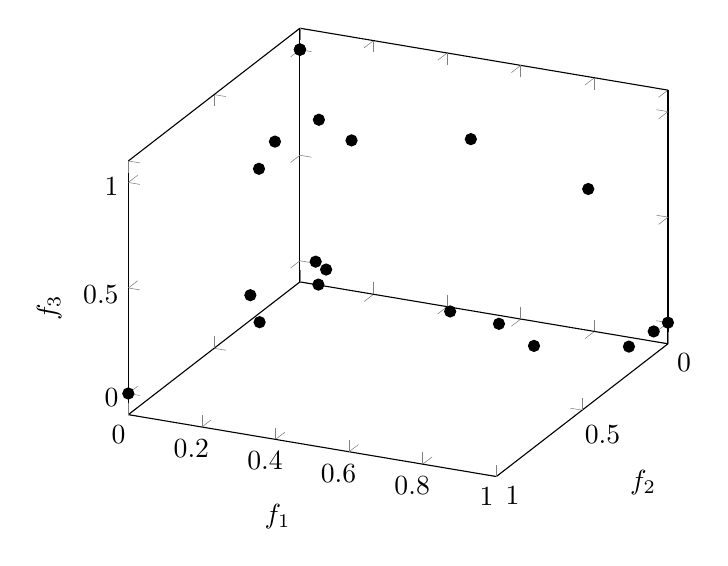
\begin{tikzpicture}[scale=1.0]
        	\begin{axis}[xlabel=$f_2$, ylabel=$f_1$, zlabel=$f_3$, view/h=115]
    			\addplot3[only marks] coordinates {
            		(1.000000, 0.000000, 0.000000) (0.000000, 1.000000, 0.000000) (0.000000, 0.000000, 1.000000) (0.000000, 0.000000, 1.000000) (0.000000, 0.000000, 1.001737) (0.036956, 0.800603, 0.598080) (0.548792, 0.144658, 0.823348) (0.317999, 0.199857, 0.926787) (0.188864, 0.982003, 0.000000) (0.854527, 0.263747, 0.451654) (0.153974, 0.536162, 0.830462) (0.356873, 0.306593, 0.884747) (0.444285, 0.139312, 0.884988) (0.769394, 0.408938, 0.490927) (0.483787, 0.861597, 0.153625) (0.729474, 0.382932, 0.566897) (0.542856, 0.793911, 0.275505) (0.885056, 0.303134, 0.354473) (0.733002, 0.413009, 0.540621) (0.076632, 0.997043, 0.005703) (0.621869, 0.698169, 0.355712) 

        		};
        	\end{axis}
	    \end{tikzpicture}
	    &
	    \begin{tikzpicture}[scale=1.0]
        	\begin{axis}[xlabel=$f_2$, ylabel=$f_1$, zlabel=$f_3$, view={45}{0}]
    			\addplot3[only marks] coordinates {
            		(1.000732,0.000000,0.000000)(0.000000,1.000821,0.000000)(0.000000,0.000000,1.000410)(0.000000,0.000000,1.000513)(0.000000,0.000000,1.018383)(0.794219,0.342283,0.503686)(0.932491,0.059257,0.360609)(0.178758,0.643231,0.746160)(0.218356,0.704885,0.678991)(0.295691,0.956651,0.051638)(0.303541,0.490835,0.819905)(0.685294,0.160561,0.711898)(0.527945,0.713948,0.471382)(0.507494,0.758125,0.413402)(0.776935,0.379386,0.504040)(0.376678,0.158927,0.918050)(0.597748,0.260002,0.760335)(0.475503,0.651285,0.593811)(0.312660,0.948571,0.113300)(0.456796,0.204828,0.868066)(0.731462,0.455115,0.540523) 

        		};
        	\end{axis}
	    \end{tikzpicture}
	\end{tabular}
    
\end{figure}

